\documentclass[aspectratio=169,11pt]{beamer}

% ============================================================
% PACKAGES
% ============================================================
\usepackage{graphicx}
\usepackage{tikz}
\usetikzlibrary{positioning,arrows.meta}
\usepackage{xcolor}
\usepackage{booktabs}
\usepackage{tabularx}
\usepackage{array}
\usepackage{ragged2e}
\usepackage{hyperref}

% ============================================================
% COLORS - SAME AS PHASE-I
% ============================================================
\definecolor{GEUBlue}{RGB}{20,55,105}
\definecolor{GEULightBlue}{RGB}{238,244,251}
\definecolor{GEUGrey}{RGB}{90,90,90}
\definecolor{GEULightGrey}{RGB}{245,246,248}

% ============================================================
% BEAMER SETTINGS
% ============================================================
\usetheme{default}
\setbeamertemplate{navigation symbols}{}
\setbeamertemplate{blocks}[rounded][shadow=false]

\setbeamercolor{normal text}{fg=black,bg=white}
\setbeamercolor{frametitle}{fg=GEUBlue}
\setbeamercolor{structure}{fg=GEUBlue}
\setbeamercolor{block title}{fg=GEUBlue,bg=GEULightBlue}
\setbeamercolor{block body}{fg=black,bg=GEULightBlue}

\setbeamerfont{frametitle}{size=\Large,series=\bfseries}

% ============================================================
% LOGO
% ============================================================
% Upload Graphic Era logo as graphicera_logo.png
\newcommand{\GEULogo}{graphicera_logo.png}

% ============================================================
% HEADER
% ============================================================
\setbeamertemplate{headline}{%
  \begin{tikzpicture}[remember picture,overlay]
    \node[
        anchor=north east,
        xshift=-0.30cm,
        yshift=-0.12cm
    ] at (current page.north east)
    {\includegraphics[height=0.62cm]{\GEULogo}};
  \end{tikzpicture}
  \vspace{0.72cm}
}

% ============================================================
% FRAME TITLE
% ============================================================
\setbeamertemplate{frametitle}{%
  \vspace{0.03cm}
  \insertframetitle\par
  \vspace{0.04cm}
  \textcolor{GEUBlue}{\rule{\textwidth}{0.9pt}}
  \vspace{0.03cm}
}

% ============================================================
% FOOTER
% ============================================================
\setbeamertemplate{footline}{%
  \leavevmode
  \hbox{%
  \begin{beamercolorbox}[
      wd=.82\paperwidth,
      ht=0.32cm,
      dp=0.10cm,
      leftskip=.3cm
  ]{author in head/foot}
    \tiny Department of Computer Science \& Engineering |
    Graphic Era (Deemed to be University)
  \end{beamercolorbox}%
  \begin{beamercolorbox}[
      wd=.18\paperwidth,
      ht=0.32cm,
      dp=0.10cm,
      rightskip=.3cm
  ]{date in head/foot}
    \hfill\tiny\insertframenumber/\inserttotalframenumber
  \end{beamercolorbox}}
}

% ============================================================
% CUSTOM COMMANDS
% ============================================================
\newcommand{\smallnote}[1]{%
\vspace{0.08cm}
{\scriptsize\color{GEUGrey}#1}
}

\newcommand{\placeholder}[1]{%
\textit{\color{GEUGrey}#1}
}

% Items the team must fill in before presenting (shown in red)
\newcommand{\fillme}[1]{\textbf{\color{red}#1}}

% ============================================================
% DOCUMENT INFORMATION
% ============================================================
\title{\textbf{Project-Based Learning}\\[2mm]\large Phase-III Evaluation}

\author{
\textbf{OptiDBX: OS--DBMS Aware Safe Online Tuning for PostgreSQL}\\
Team ID: T-021
}

\institute{
Department of Computer Science \& Engineering\\
Graphic Era (Deemed to be University), Dehradun
}

\date{Academic Session 2026--27}

% ============================================================
% DOCUMENT
% ============================================================
\begin{document}

% ============================================================
% SLIDE 1
% ============================================================
\begin{frame}[plain]

\begin{tikzpicture}[remember picture,overlay]

\draw[GEUBlue,line width=3pt]
(current page.north west) -- (current page.north east);

\node[
    anchor=north east,
    xshift=-0.45cm,
    yshift=-0.35cm
] at (current page.north east)
{\includegraphics[height=1.0cm]{\GEULogo}};

\node[
    align=center,
    text width=.84\paperwidth
] at ([yshift=.25cm]current page.center)
{
{\color{GEUBlue}
\fontsize{26}{30}\selectfont
\bfseries PROJECT-BASED LEARNING}
\\[3mm]

{\fontsize{18}{22}\selectfont
PHASE-III FINAL EVALUATION}
\\[7mm]

{\color{GEUGrey}
\Large\bfseries
OptiDBX: OS--DBMS Aware Safe Online Tuning for PostgreSQL}
\\[3mm]

{\color{GEUBlue}
\normalsize Team ID: T-021 \quad|\quad Mentor: Dr.\ Neha Tripathi}
};

\node[
    align=center,
    anchor=south,
    yshift=.42cm
] at (current page.south)
{
\bfseries
Department of Computer Science \& Engineering\\
Graphic Era (Deemed to be University), Dehradun\\[-1mm]
\scriptsize Academic Session 2026--27
};

\end{tikzpicture}

\end{frame}

% ============================================================
% SLIDE 2
% ============================================================
\begin{frame}{Team \& Mentor Details}

\begin{columns}[T,totalwidth=\textwidth]

\column{.48\textwidth}

\begin{block}{Team Information}
\begin{tabular}{@{}ll@{}}
\textbf{Team ID:} & T-021\\
\textbf{Semester:} & 5th\\
\textbf{Section:} & \fillme{XX}\\
\textbf{Domain:} & Database Systems \& Operating Systems\\
 & (Autonomous Database Tuning)
\end{tabular}
\end{block}

\column{.48\textwidth}

\begin{block}{Team Members}
1.\quad Yatharth Singh -- \fillme{Student ID}\\
2.\quad Aryaman Singh -- \fillme{Student ID}\\
3.\quad Kartikeya Kushwaha -- \fillme{Student ID}\\
4.\quad Shivansh Bhardwaj -- \fillme{Student ID}
\end{block}

\end{columns}

\vspace{2mm}

\begin{block}{Mentor}
Dr.\ Neha Tripathi
\hfill
\textbf{Interactions:} \underline{\hspace{12mm}}
\end{block}

\vfill

\smallnote{
Responsibilities: Yatharth -- tuning engine, backend \& integration;
Aryaman -- OS telemetry; Kartikeya -- DB telemetry \& decision trace;
Shivansh -- dashboard \& experiment views.
}

\end{frame}

% ============================================================
% SLIDE 3
% ============================================================
\begin{frame}{Project Abstract \& Problem Statement}

\begin{block}{Project Abstract}
\small
OptiDBX is a safety-first online tuner for PostgreSQL. Every 5\,s it pairs
OS telemetry (\texttt{/proc}, psutil) with DBMS telemetry
(\texttt{pg\_stat\_*} views), detects sustained CPU contention caused by
parallel query workers, applies \textbf{one reversible change}, measures the
effect on the workload, and \textbf{keeps it or rolls it back}. A live
dashboard shows every reading, decision and its evidence.
\end{block}

\vspace{1mm}

\begin{block}{Problem Statement}
\small
Database settings are usually tuned once, by hand. When the load changes,
too many parallel workers compete for CPU and tail latency rises, but OS tools
cannot see queries and DB tools cannot see CPU contention. Automatic tuners
that change a live system also need proof that a change actually helped.
\end{block}

\vspace{1mm}

\textbf{\color{GEUBlue}Target Users / Application}

\begin{itemize}\itemsep1pt\small
    \item DBAs and developers running self-hosted PostgreSQL
    \item Linux servers / VMs where database and other load share CPU
    \item Lower tail latency with changes that are verified and reversible
\end{itemize}

\end{frame}

% ============================================================
% SLIDE 4
% ============================================================
\begin{frame}{Objectives \& Final Deliverables}

\begin{columns}[T,totalwidth=\textwidth]

\column{.48\textwidth}

\textbf{\color{GEUBlue}Finalized Objectives}

\begin{enumerate}\itemsep3pt\small
    \item Collect paired OS + DBMS telemetry in real time
    \item Detect sustained CPU / parallel-worker contention (no false alarms on spikes)
    \item Apply one safe, reversible tuning action on owned sessions only
    \item Keep or roll back each change based on measured QPS and p95 latency
    \item Make every decision visible and explainable in a dashboard
\end{enumerate}

\column{.48\textwidth}

\textbf{\color{GEUBlue}Final Deliverables}

\begin{itemize}\itemsep3pt\small
    \item Working system: OptiDBX Safe V1 (API + live dashboard)
    \item Source code on GitHub (Python backend, React frontend)
    \item PostgreSQL telemetry store + recorded experiment traces
    \item Documentation: technical report, setup \& testing docs
    \item Research paper draft (IEEE format) on decision reliability
\end{itemize}

\end{columns}

\vfill

\smallnote{
Objectives 1--2 $\rightarrow$ telemetry modules \& detector; 3--4 $\rightarrow$
action lifecycle; 5 $\rightarrow$ dashboard; evaluation of 4 $\rightarrow$ research paper.
}

\end{frame}

% ============================================================
% SLIDE 5
% ============================================================
\begin{frame}{Phase-I \& Phase-II Feedback Incorporated}

\scriptsize

\begin{center}

\renewcommand{\arraystretch}{1.35}

\begin{tabularx}{.96\textwidth}
{@{}p{2.1cm}X X@{}}

\toprule
\textbf{Phase} &
\textbf{Feedback / Suggestion} &
\textbf{Action Taken}\\
\midrule

Phase-I &
\fillme{Feedback received during Phase-I} &
\fillme{Modification incorporated}\\

Phase-I &
\fillme{Feedback received during Phase-I} &
\fillme{Modification incorporated}\\

Phase-II &
\fillme{Feedback received during Phase-II} &
\fillme{Modification incorporated}\\

Phase-II &
\fillme{Feedback received during Phase-II} &
\fillme{Modification incorporated}\\

\bottomrule

\end{tabularx}

\end{center}

\vfill

\begin{block}{Final Improvement}
\small
Phase-I: prototype on mock data (contracts, detector, recommendation engine).
Phase-II: real OS + PostgreSQL telemetry and recommendations, no changes applied.
Phase-III: closed-loop Safe V1 -- apply, observe, keep or verified rollback,
live dashboard, evidence reports, and a measurement study of decision reliability.
\end{block}

\end{frame}

% ============================================================
% SLIDE 6
% ============================================================
\begin{frame}{Final System Architecture}

\begin{center}

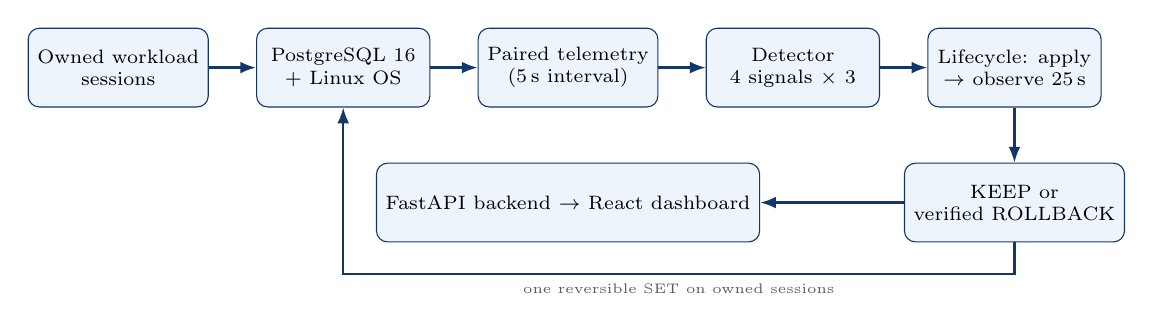
\begin{tikzpicture}[
node distance=6mm,
box/.style={
rectangle,
rounded corners,
draw=GEUBlue,
fill=GEULightBlue,
minimum width=2.2cm,
minimum height=10mm,
align=center,
font=\scriptsize
},
arrow/.style={
-{Latex[length=2mm]},
thick,
draw=GEUBlue
}
]

\node[box] (a) {Owned workload\\sessions};
\node[box,right=of a] (b) {PostgreSQL 16\\+ Linux OS};
\node[box,right=of b] (c) {Paired telemetry\\(5\,s interval)};
\node[box,right=of c] (d) {Detector\\4 signals $\times$ 3};
\node[box,right=of d] (e) {Lifecycle: apply\\$\rightarrow$ observe 25\,s};

\node[box,below=7mm of e] (f) {KEEP or\\verified ROLLBACK};
\node[box,below=7mm of c,minimum width=4.6cm] (g) {FastAPI backend $\rightarrow$ React dashboard};

\draw[arrow] (a)--(b);
\draw[arrow] (b)--(c);
\draw[arrow] (c)--(d);
\draw[arrow] (d)--(e);
\draw[arrow] (e)--(f);
\draw[arrow] (f)--(g);
\draw[arrow] (f.south) -- ++(0,-4mm) -| node[pos=0.25,below,font=\tiny,text=GEUGrey]{one reversible SET on owned sessions} (b.south);

\end{tikzpicture}

\end{center}

\vspace{1mm}

\begin{columns}[T,totalwidth=\textwidth]

\column{.48\textwidth}

\textbf{\color{GEUBlue}Major Components}

\begin{itemize}\itemsep1pt\small
    \item \texttt{os\_monitor} -- CPU, memory, disk, context switches
    \item \texttt{db\_monitor} -- \texttt{pg\_stat\_*} interval deltas
    \item \texttt{autotuner} -- detector, engine, lifecycle
    \item \texttt{backend} + \texttt{dashboard} -- API and UI
\end{itemize}

\column{.48\textwidth}

\textbf{\color{GEUBlue}System Flow}

\begin{itemize}\itemsep1pt\small
    \item Input: workload runs; both monitors sample every 5\,s
    \item Processing: 4-signal check over 3 readings
    \item Storage: metrics and actions saved in PostgreSQL
    \item Output: decision + evidence shown on the dashboard
\end{itemize}

\end{columns}

\end{frame}

% ============================================================
% SLIDE 7
% ============================================================
\begin{frame}{Final Technology Stack}

\begin{columns}[T,totalwidth=\textwidth]

\column{.48\textwidth}

\begin{block}{Software / Technologies}
\begin{itemize}\itemsep2pt\small
    \item Programming: Python 3.12, JavaScript, SQL
    \item Framework: FastAPI + Uvicorn; React 18 + Vite
    \item Database: PostgreSQL 16 (\texttt{pg\_stat\_statements})
    \item Libraries/APIs: psycopg2, psutil, Pydantic, PyYAML
    \item OS/Platform: Ubuntu 24.04 on WSL2 (Windows 11 host)
\end{itemize}
\end{block}

\column{.48\textwidth}

\begin{block}{Development Infrastructure}
\begin{itemize}\itemsep2pt\small
    \item IDE: VS Code
    \item Version Control: Git/GitHub (branches + pull requests)
    \item Testing Tools: pytest, Node test runner, Playwright
    \item Deployment: local (API :8000 in WSL, UI :3000)
    \item Other Tools: pgbench, taskset, ruff, npm/pip audit
\end{itemize}
\end{block}

\end{columns}

\vfill

\smallnote{
Why: psutil and \texttt{/proc} give OS-level signals; PostgreSQL statistics views give
query-level signals. The API runs inside WSL so it can reach PostgreSQL and the Linux
\texttt{/proc} interface directly.
}

\end{frame}

% ============================================================
% SLIDE 8
% ============================================================
\begin{frame}{Implementation of PBL Course Concepts}

\scriptsize

\begin{center}

\renewcommand{\arraystretch}{1.3}

\begin{tabularx}{.96\textwidth}
{@{}>{\bfseries}p{2.6cm}X p{3.0cm}@{}}

\toprule
Course & Concepts Actually Implemented & Project Module\\
\midrule

Operating Systems &
CPU utilisation and context switches read from \texttt{/proc}; CPU contention between
parallel worker processes; process priority (nice) and CPU affinity
(\texttt{sched\_setaffinity}, taskset) for isolation &
\texttt{os\_monitor}, \texttt{actions/os\_actions}, experiments\\

Operating Systems &
Multi-threaded workload sessions; locks for shared measurement logs;
monitor starvation under 100\% CPU and its fix by core pinning &
\texttt{workload}, \texttt{autotuner/runtime}\\

\midrule

DBMS &
Parallel query execution (Gather, \texttt{max\_parallel\_workers\_per\_gather});
session-level configuration with \texttt{SET} / \texttt{set\_config} and rollback &
\texttt{actions/db\_actions}, \texttt{autotuner/lifecycle}\\

DBMS &
Statistics views (\texttt{pg\_stat\_statements}, \texttt{pg\_stat\_database},
\texttt{pg\_stat\_activity}); SQL schema for metrics and actions;
statement timeouts; \texttt{work\_mem} temp-file spills &
\texttt{db\_monitor}, storage tables\\

\bottomrule

\end{tabularx}

\end{center}

\vfill

\begin{center}
\colorbox{GEULightBlue}{
\parbox{.88\textwidth}{
\centering
\textbf{Requirement:}
Mention only concepts that are \textbf{actually implemented}
and can be demonstrated/explained during evaluation.
}}
\end{center}

\end{frame}

% ============================================================
% SLIDE 9
% ============================================================
\begin{frame}{Module-Wise Final Implementation}

\scriptsize

\begin{center}

\renewcommand{\arraystretch}{1.3}

\begin{tabularx}{.96\textwidth}
{@{}p{2.6cm}X p{2.2cm}p{1.6cm}@{}}

\toprule
\textbf{Module} &
\textbf{Implementation} &
\textbf{Responsible} &
\textbf{Status}\\
\midrule

OS telemetry &
CPU, memory, disk and context-switch collection; storage with offline fallback;
OS health diagnostics &
Aryaman Singh &
Completed\\

DB telemetry \& decision trace &
\texttt{pg\_stat\_*} interval deltas, parallelism helpers; live 4-signal trace,
net-benefit formula and veto checklist in the UI &
Kartikeya Kushwaha &
Completed\\

Dashboard \& experiments &
Keep/rollback timeline, observation and cooldown states, \texttt{work\_mem} spill
view, multi-experiment comparison &
Shivansh Bhardwaj &
Completed\\

Tuning engine, API \& integration &
Detector, recommendation engine, journaled apply/observe/rollback lifecycle,
FastAPI routes, live sessions, evaluation study &
Yatharth Singh &
Completed\\

\bottomrule

\end{tabularx}

\end{center}

\vspace{3mm}

\begin{center}
\colorbox{GEULightBlue}{
\parbox{.75\textwidth}{
\centering
\textbf{Final Project Completion:}
\fillme{XX\%} \quad (Safe V1 complete; automatic OS tuning deferred)
}}
\end{center}

\end{frame}

% ============================================================
% SLIDE 10
% ============================================================
\begin{frame}{Working System / Prototype Demonstration}

\begin{columns}[T,totalwidth=\textwidth]

\column{.40\textwidth}

\textbf{\color{GEUBlue}Major Working Features}

\begin{itemize}\itemsep2pt\small
    \item Live session: READ / WRITE / ANALYTICAL / MIXED workloads
    \item Real-time OS + DB gauges with data provenance
    \item 6-step flow: baseline $\rightarrow$ detection $\rightarrow$ apply $\rightarrow$
          observe $\rightarrow$ decision $\rightarrow$ report
    \item Verified rollback, cooldown and recovery journal
    \item Inline algorithm flowchart; labelled simulated scenarios
\end{itemize}

\column{.58\textwidth}

\begin{block}{Live session (measured, PostgreSQL 16)}
\centering
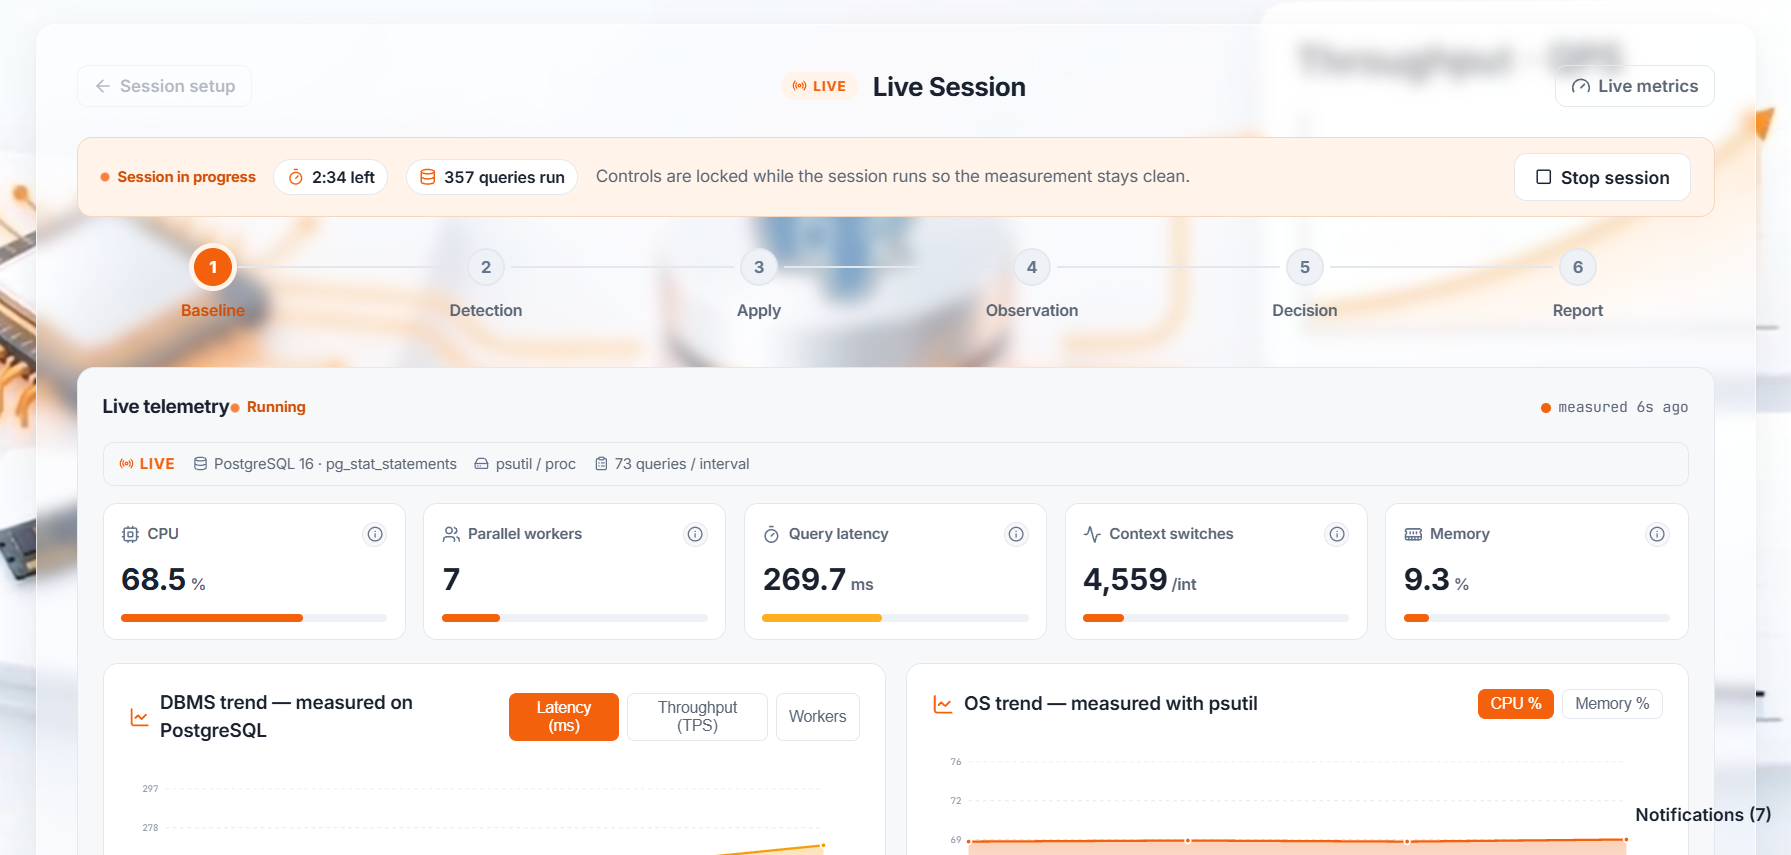
\includegraphics[width=\linewidth]{live_session.png}
\end{block}

\end{columns}

\vfill

\smallnote{
A live demonstration will be shown during evaluation; the screenshot supports it.
}

\end{frame}

% ============================================================
% SLIDE 11
% ============================================================
\begin{frame}{Data / Database / Backend Implementation}

\begin{columns}[T,totalwidth=\textwidth]

\column{.48\textwidth}

\textbf{\color{GEUBlue}Data / Database}

\begin{itemize}\itemsep2pt\small
    \item PostgreSQL 16, database \texttt{optidbx\_phase2}
    \item pgbench scale 10 ($10^6$ rows in \texttt{pgbench\_accounts})
    \item Tables: \texttt{system\_metrics}, \texttt{db\_metrics},
          \texttt{tuning\_actions}, \texttt{experiment\_runs}
    \item Interval deltas from cumulative \texttt{pg\_stat\_*} counters
    \item Validation: OS and DB readings paired only if skew $\le$ 1\,s
\end{itemize}

\column{.48\textwidth}

\textbf{\color{GEUBlue}Backend / Core Logic}

\begin{itemize}\itemsep2pt\small
    \item Detector: CPU $\ge$ 90\%, ctx-switches $\ge$ 3000, workers $\ge$ 4,
          latency $\ge$ 200\,ms, for 3 readings
    \item API: \texttt{/metrics}, \texttt{/tuner}, \texttt{/workload}, \texttt{/benchmarks}
    \item Keep rule: net = $\Delta$QPS\% $-$ 0.5$\cdot\Delta$p95\% $\ge$ 5, with vetoes
    \item Safety: only owned sessions; startup is recommendation-only
    \item Errors: statement timeouts, continuity checks, verified rollback
\end{itemize}

\end{columns}

\end{frame}

% ============================================================
% SLIDE 12
% ============================================================
\begin{frame}{Testing \& Validation}

\scriptsize

\begin{center}

\renewcommand{\arraystretch}{1.3}

\begin{tabularx}{.96\textwidth}
{@{}p{2.3cm}X X p{1.2cm}@{}}

\toprule
Test Type &
Expected Result &
Observed Result &
Status\\
\midrule

Unit + integration (pytest) &
Config, monitors, detector, lifecycle, API and safety rules behave as specified &
268 passed, 0 failed (24 Nov 2026) &
Pass\\

Dashboard (Node test runner) &
UI state models report decisions honestly; CSV export is safe &
25 passed, 0 failed &
Pass\\

System test (live) &
Full apply $\rightarrow$ observe $\rightarrow$ decision $\rightarrow$ cooldown cycle on real PostgreSQL &
Cycle completed; harmful change ($-$7.4\% QPS) rolled back &
Pass\\

Experimental validation &
Keep/rollback rule makes few wrong decisions when nothing changes &
20 runs, 46k queries: wrong KEEP in 15--40\% of replays &
Finding\\

\bottomrule

\end{tabularx}

\end{center}

\vspace{2mm}

\begin{block}{Validation Summary}
\small
Functional correctness is covered by automated tests and a live end-to-end cycle.
Decision quality was tested separately by recording real query traces and replaying
the keep rule on thousands of before/after windows; this exposed measurement
weaknesses that we report rather than hide.
\end{block}

\end{frame}

% ============================================================
% SLIDE 13
% ============================================================
\begin{frame}{Results \& Performance Analysis}

\begin{columns}[T,totalwidth=\textwidth]

\column{.46\textwidth}

\textbf{\color{GEUBlue}Key Results}

\begin{itemize}\itemsep2pt\small
    \item 6 live cycles (8 cores): 3 KEEP, 3 ROLLBACK
    \item Kept changes: QPS +4.3 to +4.5\%, p95 latency $-$5.5 to $-$8.8\%
    \item Harmful change ($-$7.4\% QPS, +8.7\% p95) correctly rolled back
    \item Trace replay: with no real change, the 25-s rule still kept it in
          15--40\% of cases; a confidence-interval gate cut adjacent-window
          errors to $\le$ 1.2\%
\end{itemize}

\column{.50\textwidth}

\begin{block}{Wrong KEEP rate vs.\ decision window}
\centering
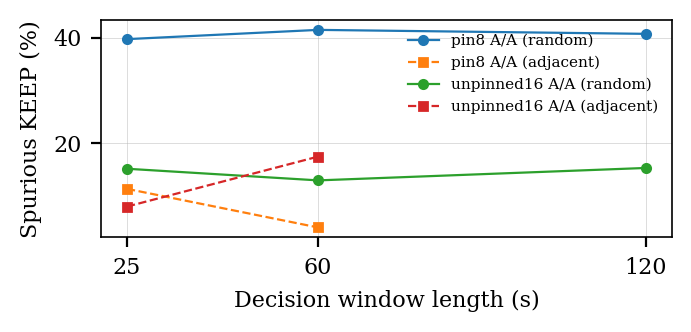
\includegraphics[width=\linewidth]{fig_window.png}
\end{block}

\end{columns}

\vfill

\smallnote{
Meaning: the tuner works, but short before/after windows can be fooled by drift
and noise -- this is the basis of our research paper and next phase.
}

\end{frame}

% ============================================================
% SLIDE 14
% ============================================================
\begin{frame}{GitHub Repository \& Development Evidence}

\begin{columns}[T,totalwidth=\textwidth]

\column{.47\textwidth}

\textbf{\color{GEUBlue}Repository Details}

\begin{itemize}\itemsep2pt\small
    \item Repository: \href{https://github.com/yathboss/OPTIDBX}{github.com/yathboss/OPTIDBX}
    \item Branch: \texttt{main} (+ feature branches per member)
    \item README.md: updated, with setup and run steps
    \item Contributors: all four members
    \item Documentation: \texttt{docs/} (report, contracts, testing)
\end{itemize}

\column{.49\textwidth}

\textbf{\color{GEUBlue}Development Evidence}

\begin{itemize}\itemsep2pt\small
    \item 143 commits on \texttt{main} since 2 Sep 2026
    \item Conventional messages (\texttt{feat:}, \texttt{fix:}, \texttt{test:})
    \item Member branches merged via pull requests
    \item Interface contracts per module in \texttt{docs/}
    \item Tests committed alongside features
\end{itemize}

\end{columns}

\vfill

\begin{center}
\colorbox{GEULightBlue}{
\parbox{.88\textwidth}{
\centering
\textbf{Requirement:}
All members must be contributors and individual development
activity should be visible through the GitHub history.
}}
\end{center}

\end{frame}

% ============================================================
% SLIDE 15
% ============================================================
\begin{frame}{Individual Contribution}

\scriptsize

\begin{center}

\renewcommand{\arraystretch}{1.3}

\begin{tabularx}{.96\textwidth}
{@{}p{2.2cm}p{2.3cm}X p{1.2cm}@{}}

\toprule
Member &
Role &
Final Technical Contribution &
Commits\\
\midrule

Yatharth Singh &
Team lead, tuning engine &
Detector and lifecycle, FastAPI backend, live sessions, module integration,
trace-replay study and paper &
129\\

Aryaman Singh &
OS telemetry &
CPU and disk collectors, OS monitor package, storage fallback, OS tests &
41\\

Shivansh Bhardwaj &
Dashboard \& experiments &
Keep/rollback visualisation, closed-loop timeline, \texttt{work\_mem} spill view,
experiment comparison &
14\\

Kartikeya Kushwaha &
DB telemetry &
DB collector interval deltas, parallelism helpers, algorithm decision-trace view &
12\\

\bottomrule

\end{tabularx}

\end{center}

\vspace{2mm}

\begin{block}{Individual Evaluation}
Every member must be able to explain, demonstrate and defend
their individual technical contribution.
\end{block}

\smallnote{
Commit counts from \texttt{git shortlog} across all branches, merging each member's
multiple Git identities.
}

\end{frame}

% ============================================================
% SLIDE 16
% ============================================================
\begin{frame}{Challenges, Limitations \& Lessons Learned}

\begin{columns}[T,totalwidth=\textwidth]

\column{.50\textwidth}

\textbf{\color{GEUBlue}Challenges \& Solutions}

\begin{itemize}\itemsep1pt\scriptsize
    \item Fake 2$\times$ gain from cold start -- exclude warm-up from baseline
    \item Stale timestamp blocked every auto-apply -- refresh at approval
    \item Monitor starved at 100\% CPU -- pin monitor to a reserved core
\end{itemize}

\vspace{1mm}

\textbf{\color{GEUBlue}Current Limitations}

\begin{itemize}\itemsep1pt\scriptsize
    \item One knob auto-tuned; OS actions are manual only
    \item Tested on one WSL2 laptop; short windows are noise-sensitive
\end{itemize}

\column{.46\textwidth}

\textbf{\color{GEUBlue}Technical Learning}

\begin{itemize}\itemsep1pt\scriptsize
    \item How OS scheduling and DB parallelism interact
    \item Measuring correctly: warm-up, paired runs, confidence intervals
    \item Safe change management: journal, verify, roll back
\end{itemize}

\vspace{1mm}

\textbf{\color{GEUBlue}Team Learning}

\begin{itemize}\itemsep1pt\scriptsize
    \item Contract-first modules let four people work in parallel
    \item Reporting negative results honestly builds trust
\end{itemize}

\end{columns}

\end{frame}

% ============================================================
% SLIDE 17
% ============================================================
\begin{frame}{Final Outcomes, Applications \& Future Scope}

\begin{columns}[T,totalwidth=\textwidth]

\column{.32\textwidth}

\textbf{\color{GEUBlue}Final Outcomes}

\begin{itemize}\itemsep2pt\small
    \item Working Safe V1 tuner + dashboard
    \item Recorded trace dataset and replay tool
    \item IEEE-format research paper draft
\end{itemize}

\column{.32\textwidth}

\textbf{\color{GEUBlue}Applications}

\begin{itemize}\itemsep2pt\small
    \item DBA assistant for self-hosted PostgreSQL
    \item Teaching OS--DBMS interaction
    \item Testing other auto-tuners' decisions
\end{itemize}

\column{.32\textwidth}

\textbf{\color{GEUBlue}Future Scope}

\begin{itemize}\itemsep2pt\small
    \item Statistical (sequential) keep rule
    \item More knobs (\texttt{work\_mem}) and TPC-H workloads
    \item Native Linux runs; automatic OS tuning
\end{itemize}

\end{columns}

\vspace{4mm}

\begin{block}{Tangible Project Outcome}
\small
A working, demonstrable prototype (OptiDBX Safe V1) plus a research contribution:
a measured study showing how often online keep/rollback decisions are wrong, being
prepared for submission to an IEEE workshop/conference.
\end{block}

\end{frame}

% ============================================================
% SLIDE 18
% ============================================================
\begin{frame}{References \& Project Resources}

\begin{columns}[T,totalwidth=\textwidth]

\column{.55\textwidth}

\textbf{\color{GEUBlue}References}

\begin{enumerate}\itemsep1pt\scriptsize
    \item D. Van Aken \textit{et al.}, ``Automatic database management system
          tuning through large-scale machine learning,'' SIGMOD 2017.
    \item X. Zhang \textit{et al.}, ``Towards dynamic and safe configuration
          tuning for cloud databases'' (OnlineTune), SIGMOD 2022.
    \item X. Zhao \textit{et al.}, ``Automatic database knob tuning: A survey,''
          IEEE TKDE, 2023.
    \item PostgreSQL 16 Documentation: Parallel Query; \texttt{pg\_stat\_statements}.
    \item Linux \texttt{proc(5)} manual; psutil documentation.
\end{enumerate}

\column{.41\textwidth}

\textbf{\color{GEUBlue}Project Resources}

\begin{itemize}\itemsep2pt\small
    \item GitHub: \href{https://github.com/yathboss/OPTIDBX}{yathboss/OPTIDBX}
    \item Demo: live, local (shown in evaluation)
    \item Dataset: \texttt{experiments/replay/data}
    \item Documentation: \texttt{docs/}, \texttt{docs/paper}
\end{itemize}

\vfill

\begin{center}

\colorbox{GEUBlue}{
\parbox{.82\textwidth}{
\centering
\color{white}
\Large\textbf{Thank You}\\[1mm]
\normalsize Questions \& Discussion
}}

\end{center}

\end{columns}

\end{frame}

\end{document}
